\section{Evaluation}
\label{sec:evaluation}

This section describes the evaluation process and presents the results of the evaluation.

Evaluation is important because:
\begin{itemize}
  \item It allows us to decide if the quality of the recommender engine archives the desired results. 
  \item We are able to compare the recommender
  \item Evaluation allows us to adjust the parameters in order to get better results.
  \item It allows us to compare different recommender techniques.
\end{itemize}


Most commonly accepted evaluation measure for recommender systems is the Mean Average Error or Root Mean Squared Error of the predicted ratings and the actual one \cite{Ricci}.

The recommender engine discussed in this article does not estimate preference values in order to produce recommendations. It presents a ordered list of $n$ recommendations.   The list is ordered from best to worst recommendation. It produces a Top-N list of recommendations. The recommenders classifies recommendable items. If we look at the recommender problem as a classification problem we can make use of precision and recall. Precision and Recall are two information retrieval concepts. We provide a brief summary here to each of these measures.

Precision and recall depend on the following measures.
\begin{description}
\item[True positive (TP)] Number of items classified as recommendable or relevant that is truly of interest to the user.
\item[True negatives (TN)] Number of instances not contained in the recommendation list (classified as irrelevant) and that in fact are not of interest to the user.
\item[False positives (FP)] Number of instances recommended but are not relevant to the user.
\item[False negatives (FN)] Number of instances not shown in the recommendation list but that in fact are relevant to the user.
\end{description}


\begin{figure}
\centering
\begin{tikzpicture}[
box/.style={draw,rectangle,minimum size=3cm,text width=2.5cm,align=left}]
\matrix (conmat) [row sep=.1cm,column sep=.1cm] {
\node (tpos) [box,
    label=left:Relevant items,
    label=above:,
    ] {relevant \\ recommendations \\ (TP)};
&
\node (fneg) [box,
    label=above:,
    label=above right:,
    label=right:] {relevant\\ but not \\recommended\\(FN)};
\\
\node (fpos) [box,
    label=left:irrelevant items,
    label=below left:,
    label=below:Top-N list] {irrelevant \\but\\recommended};
&
\node (tneg) [box,
    label=right:,
    label=below:not in Top-N list] {irrelevant\\and not\\recommended};
\\
};
\node [left=.05cm of conmat,text width=1.5cm,align=right] {\textbf{actual \\ prefences}};
\node [above=.05cm of conmat] {\textbf{recommender classification}};
\end{tikzpicture}
\caption{Confusion matrix for top-N recommendation task}
\label{fig:confusionmatrix}
\end{figure}

Figure \ref{fig:confusionmatrix} visualizes the measures used for precision and recall. This table is called confusion matrix or contingency table. 

\subsection{Precision and Recall}
\label{sec:precision}

\begin{description}
\item[Precision] Precision is the proportion of items in the top-N list of recommendatoins that are relevant \cite{Manning}.
  \begin{equation}
    \label{eq:precision}
    \text{Precision} = \frac{\text{number relevant items recommended}}{\text{size of the recommendation list}}
  \end{equation}
We can formulate this with the measures from the confusion matrix.
  \begin{equation}
    \label{eq:recallcm}
    \text{Precision} = TP/(TP+FP)
  \end{equation}

 Suppose the recommender create a list of 5 items. If 3 items are relevant recommendations then the precision is $3/5$. 
Precsion only considers the accuracy of the recommendation list and not the comprehensiveness of the result.

\item[Recall] Recall is the proportion of relevant items that appear in the recommendation result. 
  \begin{equation}
    \label{eq:recall}
    \text{Recall} = \frac{\text{number relevant items recommended}}{\text{relevant items}}
  \end{equation}
  \begin{equation}
    \label{eq:recallcm}
    \text{Recall} = TP/(TP+FN)
  \end{equation}
Suppose there are 9 relevant recommendations. If the recommender results contains 3 of these relevant recommendations then the recall is 3/9.

Note that recall should not used without precision. We could build a recommender with perfect recall by recommending all items.
\end{description}

\subsubsection{Implementation}
\label{sec:irimpl}

Listing \ref{lst:irstats} shows the implementation of precision and recall. 
The variable \verb|rec| contains an object of type \verb|Recommender|. \verb|Recommender| provides the method \verb|recommend|. \verb|recommend| takes the ID of th active user and the size $N$ of the top-N list as parameters. The argument |verb|topNsize| corresponds to $TP+FP$. It returns a top-N list for the active user. 

The variable \verb|relevantItemIDs| contains a list with relevant items for the active user.

We count how many items in the top-N list are also in the list \verb|relevantItems| and assign the result in \verb|relevantItemsRetrieved|. \verb|relevantItemsRetrieved| corresponds to the $TP$ value. In order or compute precision or recall we divide \verb|relevantItemsRetrieved| by \verb|topNsize| or the size of the collection\\ \verb|relevantItems|.

\begin{lstlisting}[caption=Implementation of precision and recall,label=lst:irstats]
double precision = 0;
double recall = 0;
int relevantItemsRetrieved = 0;

List<RecommendedItem> recItems = rec.recommend(userID, topNsize);
   for (RecommendedItem recItem : reItems) {
	if (relevantItem.contains(recItem.getItemID())){
			relevantItemsRetrieved++;
	}
   }

// Precision
int numRecommendedItems = reItems.size();
precision = ((double) relevantItemsRetrieved / (double) topNsize);
		      
// Recall
recall =  relevantItemsRetrieved / (double) relevantItems.size());
		      
\end{lstlisting}


\subsubsection{Testing Methodology}
\label{sec:relevant}

If we want to evaluate a recommender, we have to define, what is a relevant item for the active user. For the user a relevant item is one that he does not know and he would like (or purchase). Those items are unknown at the time of the recommendation. Relevancy depends on the goal of the recommender. For example, an item is relevant if the user would give it a high rating or if he would purchase the item.

Unfortunatly we do not know how a user likes some new item in the future.
But we can simulate the prefencences of the future by setting aside a small part of the real data set as test data. We split the collected input data into as follows:


We get the all ratings of user $u$. We sort these rating according the rating value. Then we select the top $N$ items $T$ from the sorted list. Items in $T$ have a high rating and we assume that it is relevant to the user $u$.
All ratings in $T$ are removed from the overall input set. The remaining preferences form the training data set $M$. 

In order to measure precision and recall we first train the recommender with the data in $M$.

We determine the top the top $N$ preferences for each user. Then we remove these values from the input data set. The resulting set is the training data set. We use this set to train the recommender engine. For instance, if we evaluate a co-occurence based recommender we compute indicator matrix from section \ref{sec:llr} with this set.

The removed entries form the test data set. Items in the test data set are the relevant items. 
For example, if $n$ is 5 this would mean precision is evaluated by removing the top 5 preferences for a user and then finding the percentage of those 5 items included in the top 5 recommendations for that user. 

The evaluatuation of the recommender can be devided into several steps:
\begin{enumerate}
\item  Compute the indicator matrix with the training set.
\item Update the search engine with the similarity values.
\item Generate a list of recommendations $r_u$ for each user.
\item Measure the precision and recall for all generated recommendations list $r$ and return the mean value.
\end{enumerate}

The evaluation process has the following parameters:
\begin{description}
\item[Size of the result] The number of recommendations to consider. The length of the recommendation list.
\item[Relevance threshold] Determines if an item is relevant or not.
\end{description}

\pgfplotsset{width=7cm}
\begin{figure}
  \centering
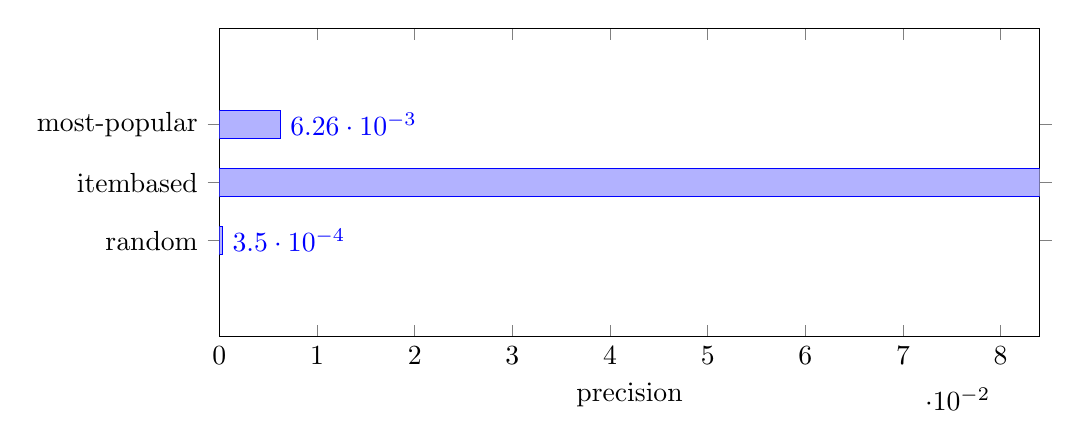
\begin{tikzpicture}
\begin{axis}[
xbar,
xmin=0,
xmax=0.084,
width=12cm,
height=5.5cm,
enlarge y limits=0.83,
xlabel={precision},
symbolic y coords={random, itembased,most-popular},
ytick=data,
nodes near coords,
nodes near coords align={horizontal},
]

\addplot coordinates {(0.00035,random) (0.00626,most-popular) (0.0864,itembased) };
\end{axis}
\end{tikzpicture} 
  \caption{Precision and recall comparison of an random generated recommendations and recommendations of itembased recommonder. The number of recommended items is 15}
  \label{fig:precisionrecallvalues}
\end{figure}

In order to get a feel what values of precision an recall to excpect we measured an itembased recommender and random generated recommendion list \cite{jannach11}.
An itembased recommender engine archives an average precision value of 0.00358. This seems a small value but if we return randomly generated recommendations we get a precision of 0.00095. Hence an itembased recommender improves the precision with a factor of 3. Figure \ref{fig:precisionrecallvalues} shows the comparison of the two measurements. We used the movielens data set for this evaluation (see section \ref{sec:dataset}).

Precision and recall has the following paramters
\begin{itemize}
\item Size of the recommendation list $N$. How many recommended items are expected. The number of items retrieved. True positives and false positives.
\item What are relevant items. Relevant items could be a threshhold in preference. Or it could be a function that return user's average preference value plus one standard deviation.
\end{itemize}

\subsection{Mahouts Evaluator}
\label{sec:mahouteval}

The library Apache Mahout provides a method to evaluate precision and recall. It is implemented in 
 \verb|GenericRecommenderIRStatsEvaluator| in the package \verb|org.apache.mahout.cf.taste.impl.eval|. The problem with this method is that the number of retrieved document $n$ is equal to the number of relevant documents and if a user has many items above threshold  \verb|GenericRecommenderIRStatsEvaluator| takes only $n$ of those. It's desirable to parameterize the definition of relevant items and number of retrieved items independently.

\begin{quote}
For each user, these implementation determine the top n preferences, then evaluate the IR statistics based on a DataModel that does not have these values. This number n is the "at" value, as in "precision at 5". For example, this would mean precision evaluated by removing the top 5 preferences for a user and then finding the percentage of those 5 items included in the top 5 recommendations for that user. 
\end{quote}

\begin{quote}
  items whose preference value is at least this value are considered "relevant" for the purposes of computations
\end{quote}

What is the impact of the parameter relevanceThreshold. According to the class description the relevant items are the users top n preferences. 

According to the description of the parameter relevanceThreshold the items whose preference is at least the threshhold are relevant. 



\subsection{Dataset}
\label{sec:dataset}

This dataset used in this project describes rating and free-text tagging activity from MovieLens, a movie recommendation service \cite{movielensdata}.
MovieLens data sets were collected by the GroupLens Research Project at the University of Minnesota.

The data was collected through the MovieLens web site (movielens.umn.edu) during the seven-month period from September 19th, 1997 through April 22nd, 1998 \cite{movielensdata}.
 
This data set consists of:
\begin{itemize}
\item 100,000 ratings. The ratings are numbers from 1 to 5. A rating is made by one user to one movie at a specific time. Each line of this file after the header row represents one rating of one movie by one user, and has the following format:
\begin{verbatim}
userId,movieId,rating,timestamp.
\end{verbatim}
\item 943 users. Each user has rated at least 20 movies
\item 1682 movies. Movies are categorized in genres. 
\item 2488 tag appliciations. A tag is applied by one user to one movie at a specific time. Tags are user-generated metadata about movies. Each tag is typically a single word or short phrase. The meaning, value, and purpose of a particular tag is determined by each user. All tags are contained in the file $tags.csv$. Each line of this file after the header row represents one tag applied to one movie by one user, and has the following format:
\begin{verbatim}
userId,movieId,tag,timestamp
\end{verbatim}
\end{itemize}

Time in the the ratings and tags set is formatted as timestamps that represends seconds since midnight Coordinated Universal Time (UTC) of January 1, 1970.

\subsection{Baseline Algorithm}
\label{sec:baselinealgorithm}

We compare the co-occurence based recommender to an item-based recommender. This section will give a brief description of item based recommenders.

\subsection{Results}
\label{sec:results}
\begin{figure}
  \centering
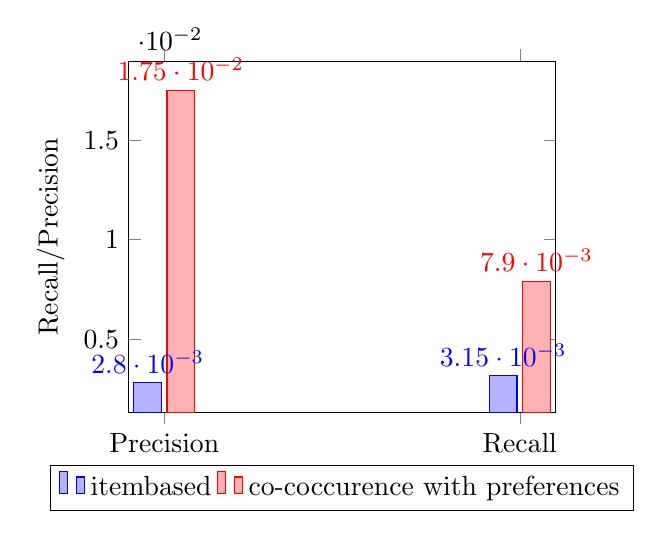
\begin{tikzpicture}
\begin{axis}[
ybar,
%enlargelimits=0.45,
legend style={at={(0.5,-0.15)},
anchor=north,legend columns=-1},
ylabel={Recall/Precision},
symbolic x coords={Precision,Recall},
xtick=data,
%ybar=5pt,% configures ‘bar shift’
%bar width=9pt,
nodes near coords,
nodes near coords align={vertical},
]
\addplot coordinates {(Precision,0.0028) (Recall,0.00315)}; 
\addplot coordinates {(Precision,0.0175) (Recall,0.0079)};

\legend{itembased,co-coccurence with preferences}
\end{axis}
\end{tikzpicture} 
  \caption{Precision and recall comparison of an item-itembased recommonder and the cooccurrence based. The result setsize is 10}
  \label{fig:results}
\end{figure}
